\subsection{Cache Memories}
\label{sec:caching}

At the time of this writing, CPU cores can process data ~200x faster than DRAM
can supply it. This gap is bridged by an hierarchy of cache memories, which are
orders of magnitude smaller and orders of magnitude faster than DRAM. This
section reviews the key concepts needed to understand \textit{cache timing
attacks} \cite{banescu2011cache}, which can be used to learn about an
application's memory access patterns. \cite{smith1982cache},
\cite{patterson2013architecture} and \cite{hennessy2012architecture} all
provide good backgrounds on low-level cache implementation concepts.

At a high level, caches exploit the high locality in the memory access patterns
of most applications to hide the main memory's (relatively) high latency. By
\textit{caching} (storing a copy of) the most recently accessed code and data,
caches can be used to satisfy 90\%-99\% of an application's memory accesses.

In an Intel processor, the \textit{first-level} (L1) cache consists of a
separate data cache (D-cache) and an instruction cache (I-cache). The
instruction fetch and decode stage is directly connected to the L1 I-cache, and
uses it to read the streams of instructions for the core's hardware threads.
Micro-ops that read from or write to memory are executed by the memory unit
(MEM in Figure~\ref{fig:cpu_core}), which is connected to the L1 D-cache and
forwards memory accesses to it.

Figure \ref{fig:cache_lookup} illustrates the steps taken by a cache when it
receives a memory access. First, a \textit{cache lookup} uses the memory
address to determine if the corresponding data exists in the cache. A
\textit{cache hit} occurs when the address is found, and the cache can resolve
the memory access quickly. Conversely, if the address is not found, a
\textit{cache miss} occurs, and a \textit{cache fill} is required to resolve
the memory access. When doing a fill, the cache forwards the memory access to
the next level of the memory hierarchy and caches the response. Under most
circumstances, a cache fill also triggers a \textit{cache eviction}, in which
some data is removed from the cache to make room for the data coming from the
fill. If the data that is evicted has been modified since it was loaded in the
cache, it must be \textit{written back} to the next level of the memory
hierarchy.

\begin{figure}[hbt]
  \center{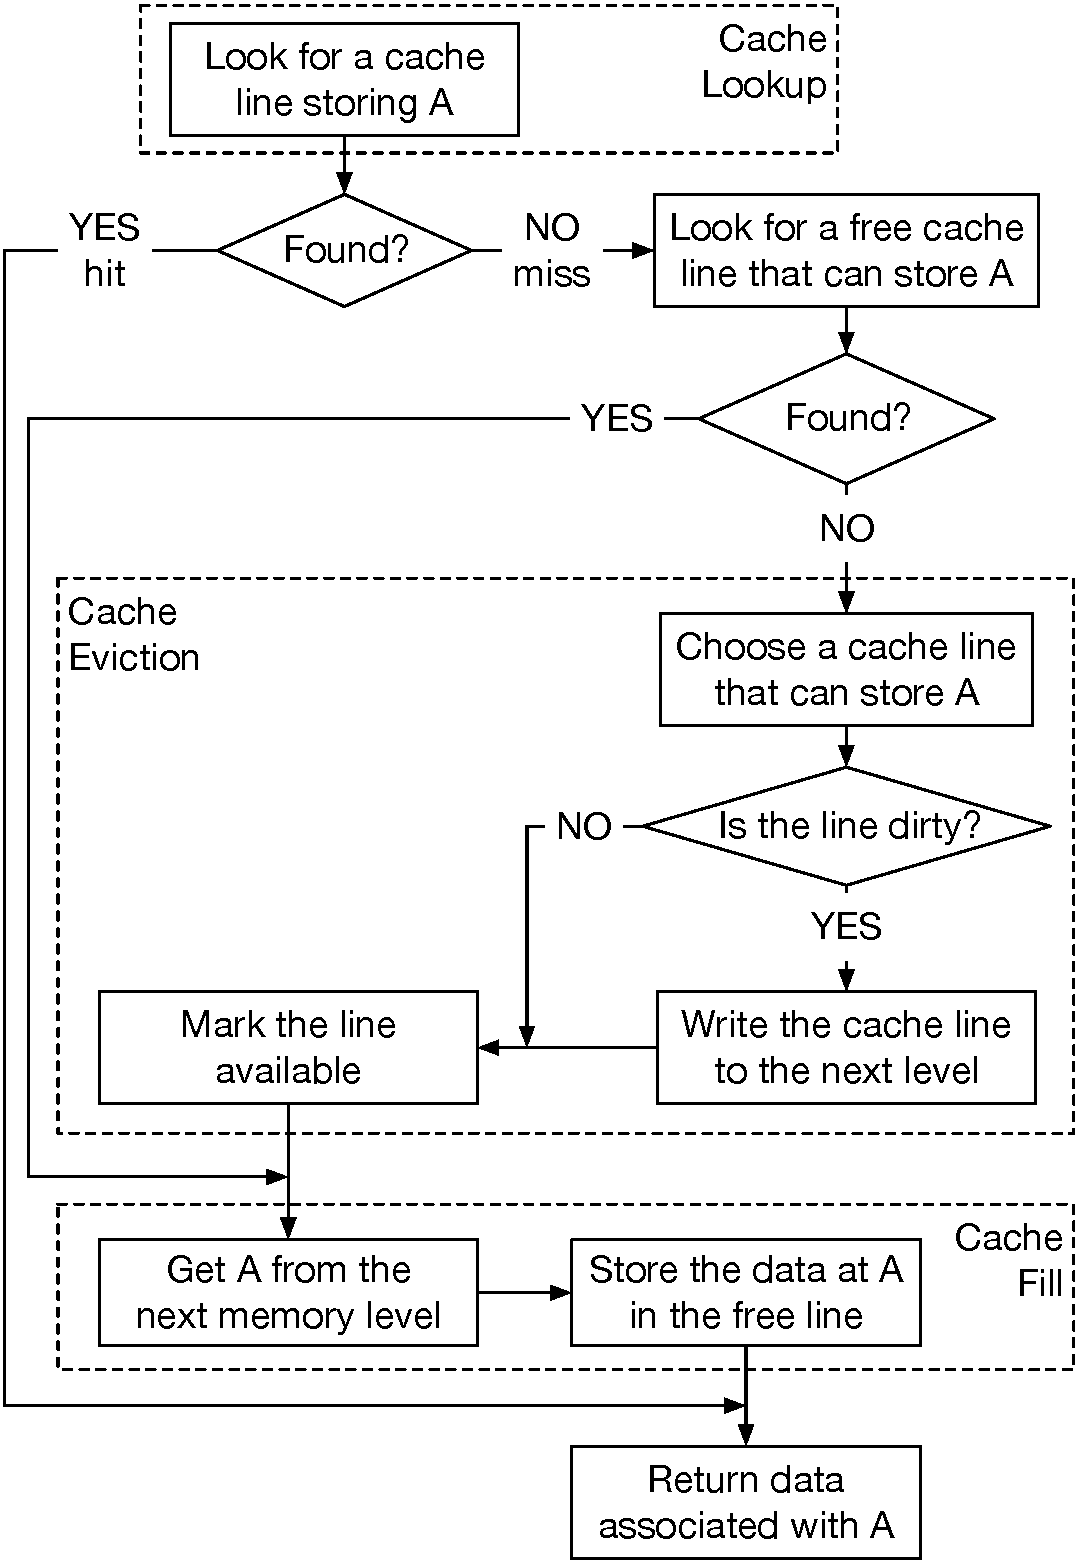
\includegraphics[width=80mm]{figures/cache_lookup.pdf}}
  \caption{
    The steps taken by a cache memory to resolve an access to a memory address
    A. An access always triggers a cache lookup. If the access misses the
    cache, a fill is required, and a write-back might be required.
  }
  \label{fig:cache_lookup}
\end{figure}

Unfortunately, caches create a dependency between the location of a memory
access and the time it takes to perform the access. A cache miss requires
at least one memory access to the next level cache, and might require a second
memory access if a write-back occurs. The related work presented in
\cite{banescu2011cache} shows that it is practical to use the timing
differences between hits and misses to learn the memory access patterns of a
target thread, as long as an attacker thread shares a cache with the target
thread. The target's memory access patterns, in turn, can reveal private
information, such as whether certain bits in an encryption key are set or not.

Table~\ref{fig:cache_timings} shows the key characteristics of the memory
hierarchy implemented by modern Intel CPUs. Each core has its own L1 and L2
cache (see Figure~\ref{fig:cpu_core}), while the L3 cache is in the CPU's
uncore (see Figure~\ref{fig:cpu_die}), and is shared by all the cores in the
package.

% Cache and Memory Subsystem: Optimization S 2.1.4
% Cache Hierarchy: Optimization S 2.2.5

\begin{table}[hbt]
  \center{\begin{tabular}{| l | r | r |}
  \hline
  \textbf{Memory} & \textbf{Size} & \textbf{Access Time}\\
  \hline
  Core Registers & 1 KB & no latency \\
  \hline
  L1 D-Cache & 32 KB & 4 cycles \\
  \hline
  L2 Cache & 256 KB & 10 cycles \\
  \hline
  L3 Cache & 8 MB & 40-75 cycles \\
  \hline
  DRAM & 16 GB & 60 ns \\
  \hline
  \end{tabular}}
  \caption{
    Approximate sizes and access times for each level in the memory
    hierarchy of an Intel processor, from \cite{intel2010perfanalysis}. Memory
    sizes and access times differ by orders of magnitude across the different
    levels of the hierarchy. This table does not cover multi-processor systems.
  }
  \label{fig:cache_timings}
\end{table}

A cache timing attack that aims at the L2 cache would have to rely on the
hypervisor or kernel to schedule a hardware thread on a logical processor in
the same core as the target software, whereas an attack on the L3 cache can be
performed using any logical processor on the same CPU. This implies that L3
cache attacks are feasible in an IaaS environment, whereas L2 cache attacks
become a possibility when running sensitive software on a user's desktop.

Our analysis of SGX concludes that it is vulnerable to cache timing attacks,
which can be used to obtain high-resolution memory access patterns for the
software running inside an SGX enclave.
